\section{En rask introduksjon til UML}
Guttorm Sindre, desember/januar 2000

Formålet med dette notatet er å gi en rask introduksjon til UML slik det skal brukes i faget Programvareutvikling og prosjektarbeidet i forbindelse med dette. Følgelig går vi ikke inn på alle deler eller detaljer ved UML, bare de som er mest relevante for faget. De som er interessert i å vite mer om UML, kan se den støttelitteraturen som er referert på slutten av dette notatet. Merk også at modelleringsmulighetene vil variere noe avhengig av hvilket verktøy man bruker. Her anbefaler vi at dere benytter Violet: http://alexdp.free.fr/violetumleditor.

\subsection{UML – hva og hvorfor?}
Vi vil også anta at sentrale begreper i objektorientert programmering, slik som klasse, metode, arv, grensesnitt, etc. er kjent fra faget TDT4100 Objektorientert programmering eller tilsvarende forkunnskaper, slik at det ikke er nødvendig å forklare disse her.

UML (Unified Modelling Language) er et objektorientert modelleringsspråk, ment brukt i analyse og design. Rundt 1990 oppsto det en rekke slike språk, med større eller mindre variasjon i konsepter og notasjon. Man så snart et behov for standardisering. Grady Booch, Ivar Jacobson og James Rumbaugh, som tidligere hadde laget hvert sitt modelleringsspråk, bestemte seg for å stikke hodene sammen, og kom opp med UML. Dette er nå blitt en slags de facto industristandard, anbefalt av OMG (Object Management Group, en organisasjon som arbeider for standardisering av objektorienterte språk og teknologier).

UML kan sies å bestå av en rekke subspråk – ulike typer diagrammer som brukes til hver sine deloppgaver i modelleringen. Hvert av disse subspråkene inkluderer visse

\begin{enumerate}

\item
\textbf{konsepter.} Akkurat som naturlige språk som norsk har ordklasser (substantiv, adjektiv, verb, etc.), vil modelleringsspråk ha ulike typer konstruksjoner som settes sammen for å lage beskrivelser av et system. Språkets syntaks (eller om man vil: grammatikk) regulerer hvordan konsepter kan settes sammen til mer komplekse uttrykk, og språkets semantikk sier noe om hva disse uttrykkene betyr. Innen hvert språk vil man dessuten ha en viss

\item
\textbf{notasjon,} dvs. en bestemt måte å skrive/vise konseptene på, f.eks. i et diagram. I mange tilfeller kan konsept og notasjon virke som to sider av samme sak, men rent formelt er det greit å skille mellom disse. Man kan godt ha flere alternative notasjoner for samme konsept. For ER-diagrammer fins det f.eks. en variant hvor attributter angis som rundinger tilknyttet entitetsklassers firkanter, og en annen variant hvor attributtene simpelthen navngis inni entitetsklassenes firkanter. Man har også eksempler på notasjon som kan bety ulike ting i ulike sammenhenger, slik som rektangler og romber – i algoritmiske flytdiagrammer betyr dette handlinger og valg, mens det i ER-diagrammer vil bety entitets- og relasjonsklasser.

\end{enumerate}

I det følgende skal vi ta for oss disse subspråkene innen UML:

\begin{enumerate}

\item
Use case diagrams

\item
Class diagrams

\item
Interaction diagrams

\item
State transition diagrams

\end{enumerate}

\subsection{Use cases}

UML inneholder ikke språk for å skrive noe som kan kalles kravspesifikasjoner. En viss modellering av brukerens interaksjon med systemet er likevel mulig, i form av use cases. Disse kan benyttes enten som en hjelp til å komme fram til en kravspesifikasjon, eller for å få bedre oversikt og forståelse for en kravspesifikasjon som allerede foreligger. Det diagrammene viser, er først og fremst hvilke funksjoner systemet skal ha, og hvilke aktører som trenger de ulike funksjonene.

\begin{figure}[H]
    \centering
    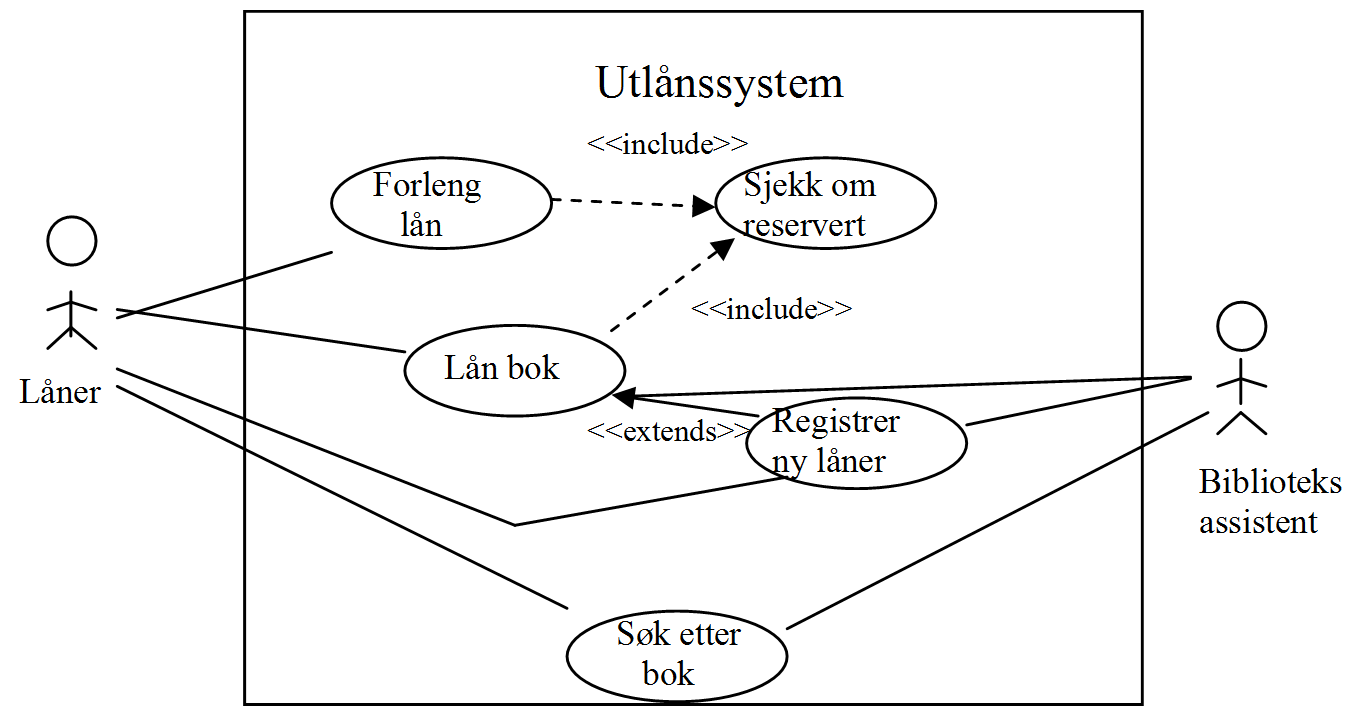
\includegraphics[scale=0.35]{resources/use-case-example.PNG}
    \caption{Use case}
    \label{fig:use-case-example}
\end{figure}

Figur \ref{fig:use-case-example} viser et Use Case for et biblioteksystem hvor kundene enten kan registrere sine lån selv via en automat, eller på mer tradisjonelt vis ved å henvende seg til en assistent. Dette er ikke et fullstendig brukstilfellediagram for systemet, man kunne også tenke seg mange andre funksjoner, f.eks. innlevering, purring, tapsmelding, erstatningskrav, …, og flere roller, f.eks. bibliotekar, som i motsetning til underordnede assistenter vil kunne foreta bestilling av nye bøker o.l. I det følgende vil vi diskutere de sentrale konseptene som der benyttet i Use Case.

\subsection{Aktør}

Aktører blir vist som menneskelignende strektegninger og skal forestille mulige brukere av systemet, med et forklarende navn (”Låner” og ”Biblioteksassistent” i diagrammet). Det er viktig å merke seg at aktøren ikke representerer en bestemt person, men en rolle overfor systemet. Flere ulike personer kan tenkes å spille samme rolle (f.eks. kan biblioteket ha 10 assistenter og tusenvis av lånere), og en og samme person kan ha ulike roller vis à vis systemet på ulike tidspunkt. En biblioteksassistent kan selv låne bøker og dermed opptre i en lånerrolle. I eksemplet er aktørene likevel enkeltpersoner (for hver enkelt interaksjon), men dette trenger ikke alltid å være tilfelle: det kan også være grupper av personer eller hele etater. Hvis systemet hadde en funksjon ”Generer årsrapport” og årsrapporten bl.a. skulle sendes til kommunen, kunne man hatt ”Kommune” som en aktør i diagrammet. I noen tilfeller kan også programsystemer figurere som aktører. Hvis biblioteket fra før av hadde et regnskapssystem og det nye utlånssystemet skulle utveksle opplysninger med dette, kunne funksjoner som innkjøp av bøker, meldinger om tap og innkreving av gebyrer ha ”Regnskapssystem” som en tilknyttet aktør.

\subsection{System}

Systemet vises som et rektangel. Dette skal forestille det automatiserte informasjonssystemet, hvis navn vil være skrevet øverst i rektanglet (her ”Utlånssystem”). Diagrammene kan brukes både til å modellere den eksisterende situasjonen eller en ønsket fremtidssituasjon. I forbindelse med programvareutvikling er ofte det siste det mest interessante, rektanglet vil i så fall indikere et system som foreløpig ikke eksisterer, men som man har tenkt å lage. Hvis man i en innledende fase er usikker på hvordan automatiseringsgrensen skal trekkes (dvs. hva som kan utføres automatisk og hva som må gjøres manuelt av mennesker), kan man starte modelleringen uten å ha noe systemrektangel og prøve å plassere dette etter hvert. Det kan også tenkes at man ønsker å modellere menneskers manuelle aktiviteter, dette må i så fall plasseres utenfor systemboksen (dog ikke særlig vanlig i UML-sammenheng).

\subsection{Use Case}

Use cases vises som navngitte oval. Vårt diagram inneholder fem ulike brukstilfeller. Et brukstilfelle kan sies å være ett tilfelle/eksempel på hvordan systemet kan brukes, én av mange funksjoner som brukerne skal tilbys. Use cases kan variere i kompleksitet. For tekstbehandling vil f.eks. ett Use Case være å slå på kursivskrift, et annet å gjøre rettskrivingskontroll på hele dokumentet. Her er det første en ytterst banal operasjon, mens det siste er langt mer komplekst og kan kreve videre interaksjon med brukeren underveis, f.eks. spørsmål om hva man skal gjøre hvis man finner feil. Et vanlig råd er at man ikke bør henge seg opp i for små og detaljerte Use Cases tidlig i modelleringen, men starte med de store og viktige først.

\subsection{Deltagelse}

Deltagelse er en relasjon mellom en aktør og et use case, vist ved en vanlig linje mellom disse to. Linjen har ingen tekst tilknyttet seg. Betydningen er at denne aktøren er involvert i dette brukstilfellet på en eller annen måte. Det kan være at aktøren tar initiativ til Use Case, altså er den som direkte ber systemet om å utføre en viss funksjon. Men koblingen kan også være løsere, f.eks. at aktøren på en eller annen måte bidrar med input eller er interessert i output fra brukstilfellet, eller på annen måte berøres av at funksjonen blir utført.

\subsection{Bruk}

Dette er rettede relasjoner mellom to brukstilfeller, vist ved piler. Betydningen er at en funksjon i systemet benytter seg av en annen funksjon. Det fins to ulike bruksrelasjoner:

\begin{enumerate}

\item
Ubetinget bruk, som innebærer at den ene funksjonen alltid vil komme til å kalle den andre. I dette tilfellet er ordet uses tilknyttet pilen, som går fra den kallende funksjonen til den kallede. Denne relasjonen er nyttig hvis to eller flere funksjoner har samme subfunksjonalitet, denne kan da skilles ut som et eget brukstilfelle som de andre kan knyttes til ved en uses-relasjon. I vårt eksempel ser vi at både ”Lån bok” og ”Forleng lån” benytter seg av ”Sjekk om reservert” – hvis en annen låner har reservert boken, kan forespørselen ikke tilfredsstilles. 

\item
Betinget bruk, som innebærer at den ene funksjonen av og til vil komme til å kalle den andre, f.eks. hvis noe går galt, slik at man må gjøre noe utover standard prosessering. I dette tilfellet er ordet extends tilknyttet pilen, som nå går fra den kallede funksjonen til den kallende. I vårt eksempel er dette tilfellet for ”Registrer ny låner”, som altså utvider ”Lån bok”. Normalt vil funksjonen ”Lån bok” ikke ha noe behov for ”Registrer ny låner”. Men hvis en person kommer og vil låne en bok, og ikke er registrert som låner ennå, må dette gjøres før lånet kan gjennomføres.

\end{enumerate}

At pilen går motsatt veg i to såpass beslektede situasjoner, er kanskje litt uheldig, men det er nå slik språket er. Hvis man ser det fra brukerens synsvinkel, kan det likevel være fornuftig. I tilfellet ”uses” er subfunksjonen alene kanskje ikke tilgjengelig eller interessant for brukeren som sådan. I diagrammet er det ingen aktør som bruker ”Sjekk om reservert” direkte, uten foranledning. Dette gjøres kun når noen er interessert i å sikre seg boken, og kan således oppfattes som en subfunksjon som ikke har interesse uavhengig av andre oppgaver. Mhp. ”extends” vil den kallede funksjonen gjerne være interessant på selvstendig basis. Vanligvis vil man jo gjøre ”Registrer ny låner” uten at man først prøver å låne en bok.

\subsection{Klassediagrammer}

Klassediagrammer er en sentral teknikk i objektorientert analyse (OOA) og design (OOD). Man kan imidlertid merke seg at begrepet OOA ikke innebærer det som enkelte andre kaller analyse (nemlig å undersøke brukernes behov og lage en kravspesifikasjon basert på dette), men å finne ut – etter at en slags kravspesifikasjon foreligger – hvilke objekter som trengs, eventuelt å få større klarhet i kravspesifikasjonen ved å undersøke hvordan den kan uttrykkes i en objektorientert modell. Kunden etterspør jo normalt ikke objekter eller klasser, men et system som tar visse typer input og leverer visse typer output innen rimelig tid, med et kurant brukergrensesnitt. For kunden spiller det gjerne ingen rolle om systemet er modellert og realisert i henhold til et objektorientert, proseduralt eller funksjonelt paradigme, så lenge det gjør jobben på en tilfredsstillende måte.

Figur \ref{fig:class-diagram-example} viser (deler av) et klassediagram for utlånssystemet diskutert tidligere. Vi vil nå forklare de sentrale konseptene basert på dette.

\begin{figure}[H]
    \centering
    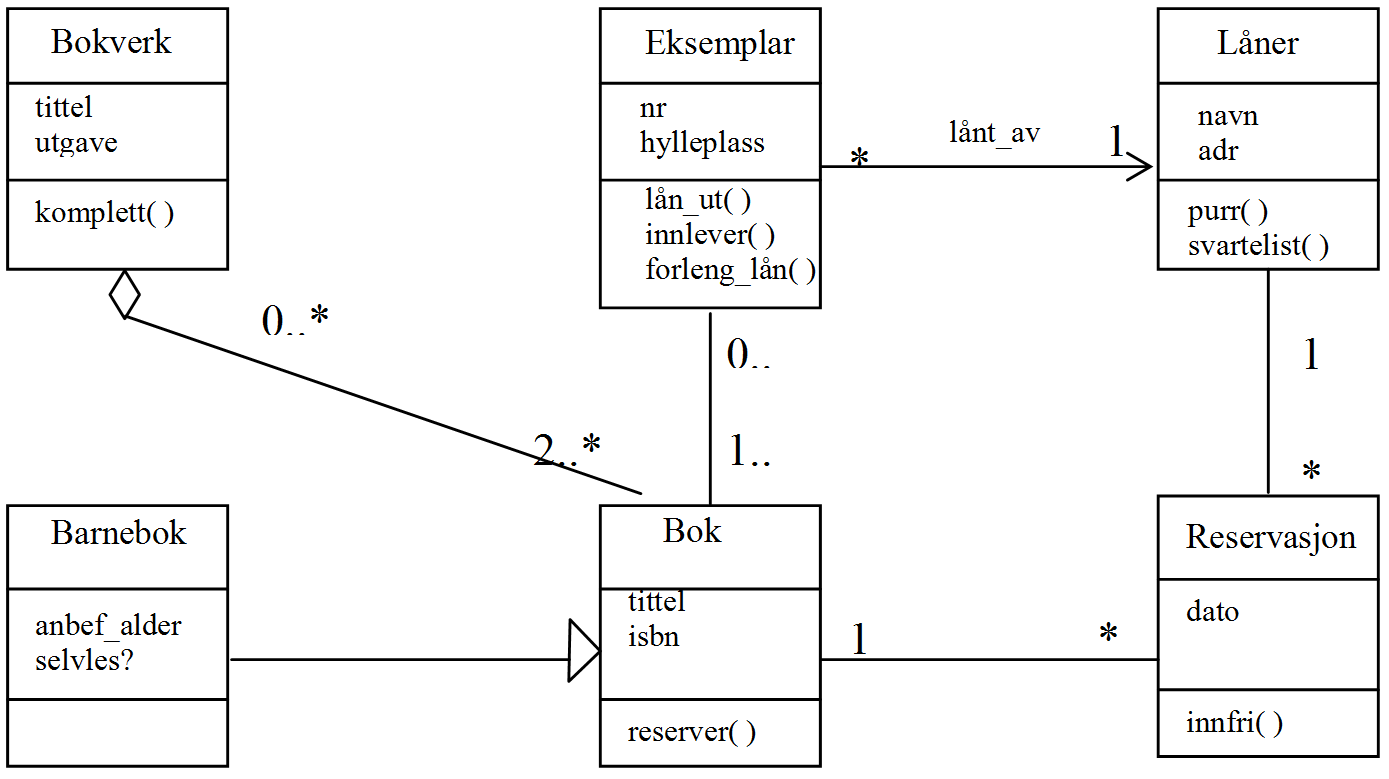
\includegraphics[scale=0.35]{resources/class-diagram-example.PNG}
    \caption{Class diagram}
    \label{fig:class-diagram-example}
\end{figure}

\subsubsection{Klasse}

Klasser vises som rektangler, med klassens navn øverst. I tillegg til navnet kan rektanglet inneholde attributter og metoder for klassen, i så fall er det vanlig å skille ut disse med horisontale delelinjer i rektanglet. Hvis man verken ønsker å oppgi attributter eller metoder, kan man droppe delelinjene. Siden en klasse kan ha et stort antall attributter og metoder, er det ofte uhensiktsmessig å nevne alle i diagrammet, i all fall på et tidlig stadium i designet, der det viktigste er å få oversikt.

De seks klassene i vårt eksempel skulle være nokså selvforklarende. Man kan merke seg forskjellen på klassene Bok, som vil være de logiske bøkene (f.eks. ”Sult” av Hamsun, ”L” av Erlend Loe) og Eksemplar, som vil være ett (av muligens flere) fysiske eksemplarer biblioteket har av boken. Det er dermed ikke bøker men eksemplarer som de facto kan lånes ut til lånere og leveres inn igjen av disse. Derimot synes det mest fornuftig at klassen Bok har metoden reserver( ). Hvis en låner ønsker å reservere f.eks. ”L”, og alle bibliotekets eksemplarer er utlånt, ønsker man normalt å få kloa i det (ukjente) eksemplaret som viser seg å bli først innlevert, ikke på forhånd å knytte reservasjonen til ett bestemt eksemplar (som kanskje aldri blir innlevert). Hvis biblioteket kun hadde ett eksemplar av hver bok, ville derimot skillet mellom Bok og Eksemplar ha vært unødvendig.

Klassen Bokverk brukes kun for verk som består av flere bind, og er utstyrt med en metode komplett( ), for å kunne sjekke om verket er komplett (dvs. biblioteket har minst ett eksemplar av alle bøker som inngår i bindet). Låner har en metode svarteliste( ), denne benyttes hvis låneren har mer enn et visst beløp utestående i gebyrer, eller har mange bøker som ikke er innlevert i tide, eller ved andre graverende forhold (f.eks. upassende oppførsel i bibliotekets lokaler). Låneren vil da ikke få låne flere bøker før det er ordnet opp i forholdet som førte til svartelistingen. 

Vårt diagram inneholder langt ifra alle attributter og metoder som ville være aktuelle, plasshensyn forhindrer oss fra å ta med alt. F.eks. måtte Eksemplar ha opplysninger om innkjøpsår og pris, når det sist ble utlånt, når det sist ble innlevert, når det sist ble vedlikeholdt. Mange av våre utelatelser er mest av plasshensyn og latskap. Men en del attributter og metoder kan det uansett være lurt å la være å nevne, i all fall på et tidlig stadium i modelleringen, der oversikt er det viktigste. Dette gjelder særlig konstruktorer, samt get- og set-metoder for nevnte attributter. Hvis man har til hensikt å lage god objektorientert design, er nemlig innlysende at slike metoder vil finnes. Når det gjelder attributter, kan man la være å nevne de som er implisitte gjennom tilbudte metoder. Siden Låner har metoden svarteliste( ), synes det unødvendig også å liste opp en attributtstatus, som kan være enten OK eller svartelistet. Attributter som er implisitte som følge av de viste relasjonene (se kommentar nedenfor), kan også gjerne utelates, i all fall på et tidlig stadium.

\subsubsection{Relasjoner}

Relasjoner mellom klassene uttrykker sammenhenger mellom disse. Det fins tre hovedtyper slike relasjoner:

\begin{enumerate}

\item
Vanlige (assosiative) relasjoner

\item
Generalisering

\item
Aggregering

\end{enumerate}

I det følgende vil vi ta for oss hver av disse i mer detalj.

A) Vanlige (assosiative) relasjoner. Disse vises ved enkle linjer, uten noen spesiell symbolbruk, annet enn eventuelt vanlige strekpiler i enden for å vise navigasjonsretningen. I vårt eksempel har vi stort sett latt vær å angi navigasjonsretningen, den er kun med for forholdet mellom ”Eksemplar” og ”Låner”, pilen indikerer her at vi fra et eksemplarobjekt direkte vil kunne finne det tilhørende lånerobjektet, men ikke omvendt. Implementasjonsmessig vil dette bety at eksemplaret har en attributt med referanse til et lånerobjekt. Vi kunne også ha valgt det motsatte, nemlig at hvert lånerobjekt inneholdt en liste med referanser til de eksemplarobjekter låneren p.t. hadde i sin besittelse. Eller man kunne gjort begge deler, og dermed hatt muligheten til å navigere begge veier (fordel med hensyn på raskere navigering, ulempe fordi man får redundans i datastrukturen, noe som vil gi langsommere oppdatering og større fare for feil). Hvilken variant man velger vil avhenge av hva slags funksjonalitet brukerne vanligvis etterspør, og med hvilke effektivitetsbehov. Normalt vil det lønne seg å utsette inngående vurderinger av navigasjonsretning til man har fått klarhet i hvilke klasser og relasjoner man skal ha. Enkel linje (uten noen piler) betyr altså at navigasjonsretningen foreløpig ikke er bestemt, mens dobbel navigasjonsretning vil bli vist ved at man har pil begge veier.

Hvis det er tvil om betydningen av en relasjon, bør den også navngis. I vårt eksempel anses relasjonene for selvforklarende, men vi har likevel vist navngiving mellom Eksemplar og Låner. Nær endene av hver relasjonslinje vil man finne opplysninger om relasjonens kardinalitet, à la hva man har for ER-diagrammer. Man kan for det første angi om en relasjon er til-en (1) eller til-mange (*). Hvis man ønsker det, kan man også angi om deltagelse i relasjonen er obligatorisk eller frivillig (1..1 eller 1..* vil signalisere obligatorisk deltagelse, mens 0..1 eller 0..* signaliserer frivillig deltagelse). Frivillig/obligatorisk kan anses som et mer detaljert spørsmål enn en/mange, man bør derfor få klarhet i det siste først.

Vi ser fra diagrammet at en låner kan ha lånt flere eksemplarer (*), men hvert eksemplar vil kun være lånt av en låner av gangen (1). Et eksemplar vil kun være eksemplar av én bok (1..1), og det må også være eksemplar av en bok (1..1). Derimot kan bøker finnes i mange eksemplarer (0:*), og det kan finnes bøker vi ikke har noen eksemplarer av (0:*). I dette siste tilfellet kan det kanskje synes rart at man fortsatt ønsker å ha opplysninger om boken lagret i systemet, men dette kan være interessant i noen situasjoner, f.eks. hvis det er en bok som er blitt mistet og som var del av et større bokverk, hvilket vil tilsi et sterkt incentiv for å prøve å skaffe seg boken igjen, og dermed komplettere bokverket.

B) Generalisering. Mange kaller denne relasjonen for arv eller arving. Navnet på selve den konseptuelle relasjonen er imidlertid generalisering, eventuelt den inverse spesialisering, mens arving mer er en mekanisme i objektorienterte programmeringsspråk. Dvs., man kan godt tenke seg modelleringsspråk hvor man kan uttrykke generalisering, uten at det dermed fins en arvemekanisme. I mengdealgebraisk forstand kan generalisering sies å tilsvare en overmengderelasjon (superset). Hvis vi alltid har $ A \supset B $, er $ A $ en generalisering av $ B $, dvs. ethvert element i $ B $  vil også være medlem i $ A $. I objektorientert sammenheng snakker man om superklasse (den generelle) og subklasse (den spesialiserte).

I vårt eksempel er ”Barnebok” en subklasse av ”Bok”, dette vises ved et trekantsymbol ved superklassen og en linje derfra til subklassen. Motivasjonen for å skille ut barnebøker i en spesiell subklasse, kan være at de har spesielle attributter eller metoder som ikke er aktuelle for bøker flest, som her anbef\_alder og selvles? – den siste indikerer om barn i anbefalt alder kan antas å lese boken på egen hånd, eller om den må leses høyt av en voksen. Barnebøker vil også være plassert i en egen avdeling i biblioteket, og det kan være andre regler med hensyn på frister og antall man kan låne på en gang.

I figur \ref{fig:class-diagram-example} har superklassen bare en subklasse, men ofte vil det være flere alternative subklasser. Da vil man knytte alle disse til det samme trekantsymbolet. I mer avanserte tilfeller kan en og samme superklasse være generalisering for flere uavhengige subklassehierarkier på samme tid, da vil man også trenge flere trekantsymboler ved samme klasse. Figur \ref{fig:orthogonal-generalization-hierarchy-example} viser et eksempel hvor vi har flere ortogonale (dvs. uavhengige) dimensjoner som bøker kan spesialiseres etter, på den ene siden ”Barnebok” og ”Ungdomsbok”, på den andre siden ”Lånbar bok” og ”Ikke-lånbar bok” (f.eks. oppslagsverk som det ikke er lov å ta ut av biblioteket). I dette tilfellet annoterer man hver generaliseringstrekant med en viss rolle, her ”aldersgruppe” og ”lånbarhet”. Sistnevnte rolle er markert med {complete}, dette betyr at enhver bok må være enten lånbar eller ikke-lånbar. For ”aldersgruppe” fins ingen slik markering, altså vil man også kunne ha bøker som verken er barnebøker eller ungdomsbøker (f.eks. voksenbøker, som man ikke har sett det hensiktsmessig å lage noen egen klasse for).

\begin{figure}[H]
    \centering
    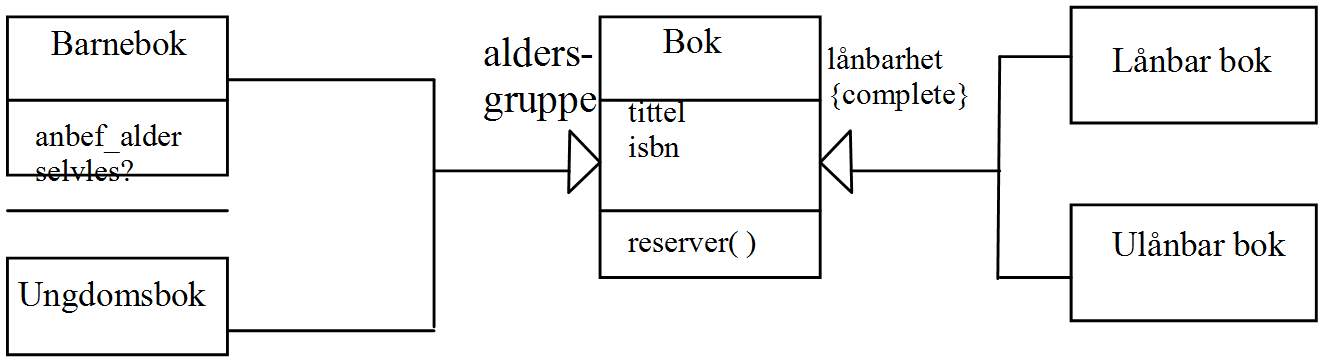
\includegraphics[scale=0.35]{resources/orthogonal-generalization-hierarchy-example.PNG}
    \caption{Two orthogonal generalization hierarchies}
    \label{fig:orthogonal-generalization-hierarchy-example}
\end{figure}


I noen tilfeller kan man ønske å gjøre superklassen abstrakt, hvilket innebærer at alle objekter som tilhører klassen også tilhører en eller annen av dens subklasser, slik at man ikke har til hensikt å instansiere objekter av selve superklassen. Dette kan markeres ved å sette nøkkelordet {abstract} høyrejustert under klassens navn, eventuelt også sette navnet i kursiv. Grensesnitt kan markeres nesten på samme måte som abstrakte klasser. Man bruker samme trekant som for generalisering under rektanglet for grensesnittet, og setter også her navnet i kursiv, men skriver nå nøkkelordet ”interface” venstrejustert over navnet. Dessuten er linjen fra trekanten til rektanglet for implementerende klasser stiplet. Av plasshensyn viser vi ikke eksempler på disse tingene. Abstrakte klasser og grensesnitt bør være forstått fra Programmeringsfaget, og spesielt interesserte kan eventuelt oppsøke mer inngående litteratur om UML for eksempler.

C) Aggregering. Denne relasjonen uttrykker at deler settes sammen til en større helhet, i invers forstand ofte kalt en ”part-of” relasjon. Hvis A er en aggregering av B og C, uttrykker dette i mengdealgebra at $ A \subset B \times C $, dvs. at A er en undermengde av det kartesiske produktet av B og C. Det kartesiske produktet gir alle mulige kombinasjoner av de to operandene. Hvis f.eks. B er HTML-hoder (alle eksisterende tekststrenger \textless HEAD\textgreater … \textless HEAD\textgreater ) og C er HTML-kropper (alle eksisterende tekststrenger \textless BODY\textgreater …\textless /BODY\textgreater ), vil det kartesiske produktet være alle mulige kombinasjoner hvor et hode settes sammen med en kropp. Mange av disse kombinasjonene vil ikke tilsvare eksisterende websider (selv om man i noen tilfeller kan tenke seg samme kropp eller samme hode duplisert flere steder). Nettopp derfor er det viktig å få med undermengdetegnet: Hvis A er klassen av websider vil det være riktig (hvis vi ser bort fra en del komplikasjoner, f.eks. at man også kan ha FRAMESET istf. BODY) å si at denne er et subsett av det kartesiske produktet.

I vår Figur \ref{fig:class-diagram-example} er aggregering brukt for å vise at et bokverk består av et antall bøker. For aggregering bruker UML et rombeformet symbol under helhetsklassen, med koblinger til delklassen(e). I dette tilfellet, hvor det bare er én delklasse og vi har kardinalitetsuttrykket 2..* på Boksiden av relasjonen, sier modellen at et bokverk består av minst 2, muligens flere, bøker (dvs. $ Bokverk \subset Bok \times … \times Bok $). På bokverksiden av relasjonen står det 0..*. Biblioteket kan godt ha bøker som ikke er med i noe bokverk (vanligvis de fleste). *-tegnet impliserer at en bok faktisk også kan være med i flere bokverk på en gang (f.eks. at Hamsuns ”Sult” kan være representert både i ”Hamsuns samlede” og ”Norske klassikere”). 

Man kan godt tenke seg eksempler hvor flere delklasser er tilknyttet samme aggregering (en webside består av et hode og en kropp; en bil består av karosseri, chassis, motor, eksosanlegg, et antall hjul, etc.). I slike tilfeller kan man knytte flere delklasser til samme aggregeringsrombe, nettopp som man knyttet flere alternative subklasser til samme trekant for generalisering. Man kan også tenke seg muligheten av å dekomponere samme helhet på flere ortogonale måter. På den ene siden kan et menneske tenkes å bestå av hud, hår, skjelett, tenner, negler, muskler, blod, etc. (dekomponering i henhold til materialtype), på den annen side av hode, torso, armer, ben etc. (dekomponering i henhold til kroppsdel).

I UML fins det to forskjellige aggregeringsrelasjoner. Den ene kalles simpelthen aggregation, og vises ved hvitt rombesymbol, som brukt i vår figur. Den andre kalles composition, med samme rombesymbol, bare at det nå er fylt med svart. Betydningen er den samme, bortsett fra at composition-relasjonen har noen tilleggskrav:
Ethvert delobjekt kan kun tilhøre én helhet. I vårt eksempel så vi en mulighet for at en bok kunne tilhøre flere bokverk på samme tid, dermed passet ikke ”composition” i dette tilfellet. Men svært ofte når det er snakk om aggregering, vil kravet om kun én helhet være implisitt. Et hjul kan f.eks. kun befinne seg på en bil av gangen.
Delene er forventet å være avhengige av helheten for å eksistere. Dvs., hvis helheten forsvinner, så forsvinner også alle dens deler. I data(base)sammenheng vil dette innebære at man bruker kaskadesletting for delene dersom helheten blir slettet. Men kanskje er heller ikke dette ønskelig i vårt eksempel. Hvis man i utgangspunktet har et bokverk bestående av syv bøker, og så mister fem av dem, ville det kunne være aktuelt å slette bokverket (dvs. at datasystemet ikke lenger skal oppfatte det som om dette innehas av biblioteket). Normalt vil man likevel ikke ønske å kaste de enkeltbøkene man fremdeles er i besittelse av, men beholde disse som frittstående bøker.

Altså passer det ikke å bruke composition i vårt eksempel, og vi nøyer oss med vanlig aggregation. Men man kan lett tenke seg andre eksempler hvor det ville passe, f.eks. hvis en ordre består av et antall ordrelinjer (linje 1: 1000 eks av varenummer 24, linje 2: 500 eks av varenummer 56, etc.). Om man da sletter selve ordren, vil man også ønske å slette alle dens ordrelinjer, siden disse ikke kan eksistere uavhengig av noen ordre. Og i dette tilfellet ville en ordrelinje bare kunne være del av én ordre. Selv om det tilfeldigvis fantes to forskjellige kunder som begge hadde bestilt 1000 eks av varenummer 24, ville man likevel ikke si at dette var samme ordrelinje, men to forskjellige ordrelinjer med samme verdi for varenummer- og antall-attributtene, akkurat som det også kan finnes personer med samme navn, samme høyde etc., uten at disse dermed er den samme personen).

Det er viktig å være klar over forskjellen på generalisering og klassifisering. Generalisering er et forhold mellom to mengder (eller i objektorientert forstand: mellom to klasser), og forteller at den ene er en undermengde (subklasse) av den andre. Klassifisering er derimot et forhold mellom individ (enkeltobjekt) og klasse. Generalisering: En barnebok er en bok. Klassifisering: ”Sult” er en bok. Det som kan lure enkelte, er at frasen ”er en” kan benyttes i begge sammenhenger. Men i det første tilfellet er det generelle substantiv (fellesnavn) både foran og bak, mens det i det andre tilfellet begynner med et særnavn (bokens tittel). Om man skulle klassifisere videre fra ”barnebok” heller enn å generalisere, ville man ikke komme til ”bok”, men få barnebok er et substantiv eller barnebok er et begrep – med klassifisering klarer man kun et par transitive ledd før man ender opp i ekstremt abstrakte konsepter.

Det er også viktig å skjønne forskjellen på generalisering og aggregering, som noen har en lei tendens til å forveksle. Generalisering brukes som en relasjon mellom et generelt begrep og et mer spesielt begrep. Et objekt av subklassen kan også sies å være medlem av superklassen, men ikke nødvendigvis omvendt. Aggregering brukes derimot som en relasjon mellom noe stort og noe mindre som dette store består av. I dette tilfellet vil ikke et objekt av en av delklassene også være et eksempel på et objekt av den overordnede klassen (et hjul er ikke en bil). For generalisering kan man som nevnt lage fornuftige setninger av typen ”En/et <subklasse> er en/et <superklasse>”, f.eks. ”En barnebok er en bok” (pass på å ha med artikler en/et, dette forhindrer forveksling med klassifisering). Prøver man derimot ”En bok er et bokverk”, eller ”Et bokverk er en bok”, vil forhåpentligvis de fleste føle motvilje. For aggregering kan man lage setninger som ”En/et <aggregatklasse> består av <delklasser> (hvor man bruker entall for delklassenavnet hvis kardinaliteten er 1, flertall hvis den er mange)”, f.eks. ”Et bokverk består av bøker”, ”En bil består av karosseri, chassis, motor, lykter, hjul…” Om man prøver med ”En bok består av barnebøker” eller ”En barnebok består av bøker”, vil man forhåpentligvis merke at noe ikke stemmer…

Et mer kinkig problem kan være å skjønne forskjellen på aggregering og vanlige assosiative relasjoner. Forholdet mellom Bokverk og Bok kunne også ha blitt modellert som en vanlig en-til-mange relasjon (eller i vårt tilfelle faktisk mange-til-mange, siden vi tillater bøker å være med i flere bokverk samtidig). I og for seg ville det ikke ha vært noe galt i dette, man kunne ende opp med en helt kurant design, siden kodingen godt kan bli den samme om man hadde aggregering eller vanlig assosiativ relasjon. Men konseptuelt sett blir modellen mindre informativ hvis man unnlater å bruke aggregering når det egentlig er dette man har. Med en vanlig relasjon mellom bokverk og bok ville vi ikke se noen fundamental forskjell på denne og øvrige relasjoner i diagrammet, f.eks. mellom låner og reservasjon. Men normalt ville man ikke oppfatte reservasjonene som en del av den respektive låneren, og om en reservasjon slettes, ville man ikke si at låneren som sådan hadde forandret seg. Hvis derimot en av bøkene i et bokverk går tapt for biblioteket, er bokverket som helhet blitt redusert (til et ”innkomplett bokverk”). På spørsmålet ”Har dere en låner som heter Kari Karinesdatter?” ville systemet eller bibliotekspersonellet uten videre kunne svare ja, såframt denne var registrert og den som spurte hadde rett til å få opplysningen – også om den nevnte Kari p.t. ikke hadde noen løpende reservasjoner eller lån. På spørsmålet ”Har dere Hamsuns samlede?” kunne det derimot innvendes at et ubetinget ”Ja” ville være galt svar, eller iallfall misvisende, hvis det faktisk var slik at noen av bindene var gått tapt. Da ville et korrekt svar snarere være ”Ja, men vi mangler bind 5 og 7.”– eller hvis mange av bindene manglet, kanskje til og med ”Nei, vi har bare de to første bindene.” En modell hvor man har et korrekt skille mellom vanlige assosiative relasjoner og aggregering/komposisjon, vil derfor gi bedre innsikt i forholdet mellom de involverte klassene.

\subsection{Sekvensdiagrammer}

Sekvensdiagrammer (sequence diagrams) har som mål å vise hvordan flere objekter samarbeider for å løse en bestemt oppgave. En ”oppgave” i denne sammenhengen vil typisk tilsvare ett brukstilfelle. I figur \ref{fig:two-sequences-one-diagram-example} er det vist to enkle sekvenser i det samme diagrammet. Her får vi illustrert både hvordan man viser metodekall mot eksisterende objekter, nyskaping av objekter og sletting av objekter. De sentrale konseptene i sekvensdiagrammet vil bli forklart i de følgende delkapitler.

\begin{figure}[H]
    \centering
    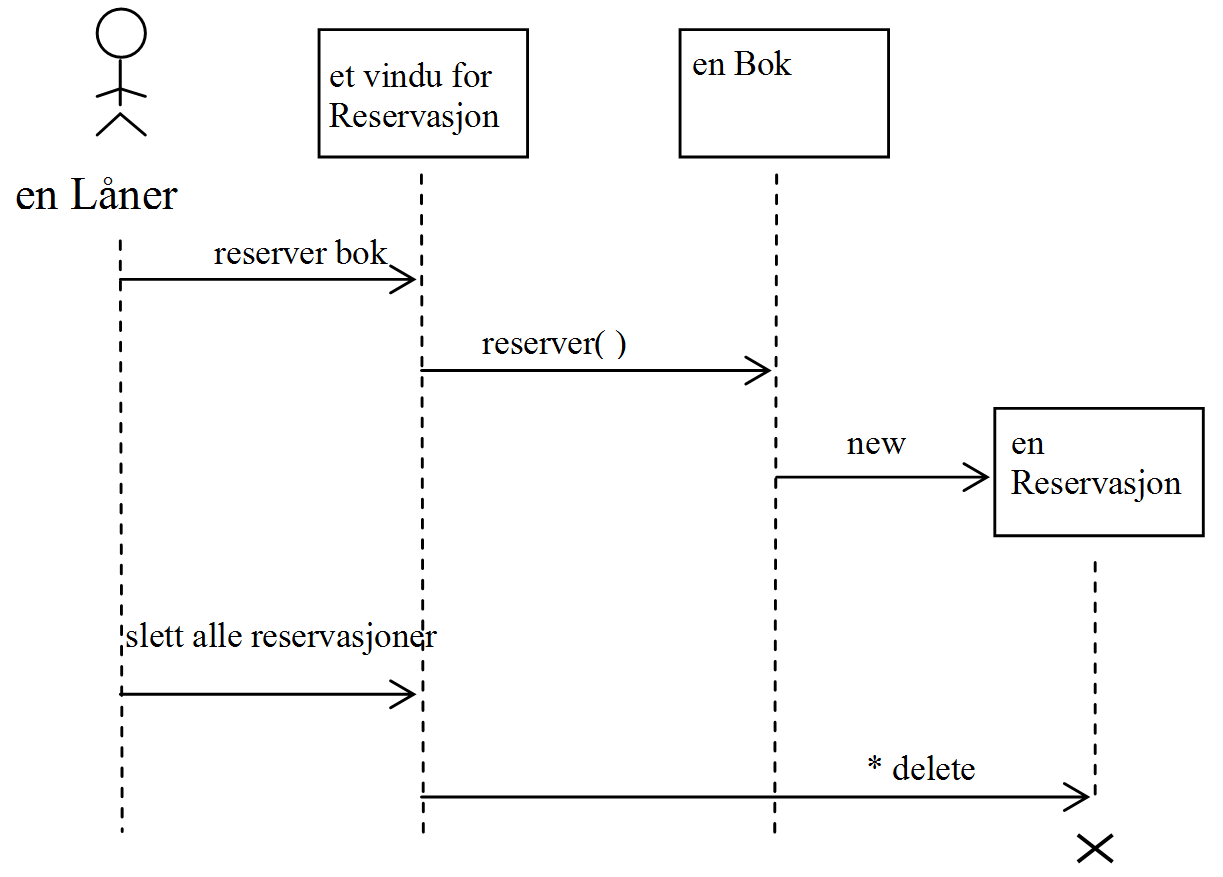
\includegraphics[scale=0.35]{resources/two-sequences-one-diagram-example.PNG}
    \caption{Two sequences in the same diagram}
    \label{fig:two-sequences-one-diagram-example}
\end{figure}

\subsubsection{Objekter}

Objekter vises ved navngitte rektangler som i utgangspunktet plasseres øverst i diagrammet. At det står ”en Bok”, ”en Reservasjon” etc., signaliserer nettopp at det her ikke dreier seg klasser, men om enkeltobjekter av klassene. Hvis man vil kan man også ha med aktører på linje med objektene for å vise hvordan handlingssekvensene initieres ved eksterne kommandoer fra brukeren. Aktørene er vist ved samme notasjon og har samme betydning som før, og vi vil ikke diskutere dem nærmere her, mange bruker dem heller ikke i sekvensdiagrammene. Den observante leser vil ha merket seg at vindusobjektet (det lengst til venstre) ikke er inkludert i klassediagrammet vårt i figur \ref{fig:orthogonal-generalization-hierarchy-example}. Dette objektet er av en klasse som er del av brukergrensesnittet. Det er ikke noe i veien for å ha med slike objekter i klassediagrammene (tvert imot, de bør modelleres på et eller annet tidspunkt i utviklingen), men vi droppet for enkelthets skyld alle tanker på dette i figur \ref{fig:class-diagram-example} for å konsentrere oss om den konseptuelle siden ved biblioteksdomenet.

Hvert objekt vil være utstyrt med en livslinje, nemlig den stiplede linjen som går loddrett nedover fra hvert objekt. Disse indikerer objektets levetid, og står som et tilknytningspunkt for meldinger. I noen varianter av sekvensdiagrammer bruker man en mer detaljert notasjon hvor det er uthevede partier på livslinjen i de perioder det tilhørende objektet er aktivt, men dette er droppet her. Når det gjelder rekkefølgen på hendelser skal livslinjene leses ovenfra og ned. Et kryss på livslinjen betyr at objektet opphører å eksistere.

\subsubsection{Meldinger}

Meldinger vises ved piler mellom livslinjene, annotert med meldingens navn. En * foran meldingsnavnet betyr at meldingen kan bli repetert mange ganger. I noen tilfeller kan en melding gå rett til en objektboks i stedet for til dets livslinje, dette brukes når dette objektet blir opprettet (med new).

I figur \ref{fig:two-sequences-one-diagram-example} ser vi først at låneren gir en kommando om å reservere en bok (f.eks. ved å fylle inn opplysninger om forfatter og tittel og klikke på en ”Reserver”-knapp på skjermen). Dette fører til at vindu-objektet sender en reserver()-forespørsel til det aktuelle bok-objektet. Her ser vi for enkelhets skyld bort fra komplikasjoner som kunne føre til at reservasjonen ble avvist. Det fortsetter dermed betingelsesløst med at bok-objektet utfører en new-operasjon som oppretter et reservasjonsobjekt.

I den neste sekvensen, som er satt sammen med den første så vi skal slippe å tegne så mange bokser, bestemmer en låner seg for å slette alle sine reservasjoner. Dette vil føre til en repetert (*) delete-operasjon mot diverse reservasjonsobjekter, og disse opphører å eksistere som følge av handlingen.

\subsubsection{Betingelser}

For mer presis modellering kan man både angi parametere og dessuten utstyre meldingene med betingelser, angitt i [ ]-parenteser. Hvis en betingelse er angitt, betyr dette at meldingen kun vil bli sendt dersom betingelsen er tilfredsstilt. Et eksempel med bruk av betingelser er vist i figur \ref{fig:sequence-diagram-with-conditions-example}.

\begin{figure}[H]
    \centering
    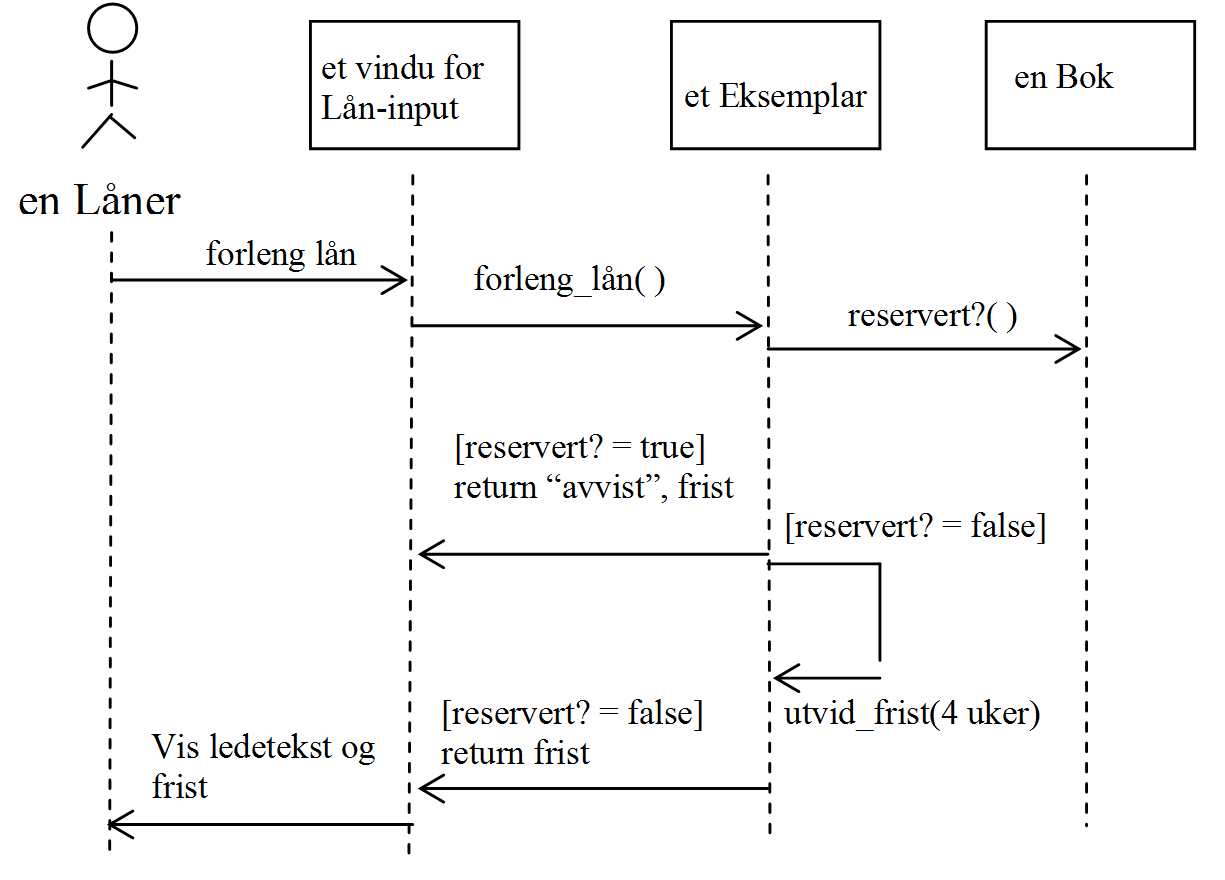
\includegraphics[scale=0.35]{resources/sequence-diagram-with-conditions-example.PNG}
    \caption{Sequence diagram with conditions}
    \label{fig:sequence-diagram-with-conditions-example}
\end{figure}

I figur \ref{fig:sequence-diagram-with-conditions-example} gir en låner inn et ønske om å forlenge lånet av et eksemplar, dvs. å få utsatt innleveringsfristen. La oss anta at bibliotekets policy på dette er at man standard får 4 ukers utsettelse, såfremt boken ikke er reservert av noen andre. Vinduet sender en forleng\_lån( )-melding til det aktuelle eksemplar-objektet. Eksemplar-objektet må så sende en reservert?( )-melding til det tilhørende bok-objektet, denne vil mest hensiktsmessig returnere true eller false. Nå kommer bruken av betingelser inn i bildet. Hvis boken var reservert, må forlengelsen avvises. Ellers er det i orden å forlenge lånet. Eksemplar-objektet sender da meldingen utvid\_frist(4 uker) til seg selv (dvs. kaller en metode i samme objekt), dette kalles selv-delegering (self-delegation). For de øvrige metodekallene har vi ikke inkludert parametere, enten fordi de ikke trengs, eller fordi de antas å være innlysende. Her har vi også valgt å vise hvordan resultater returneres, noe som ofte ikke gjøres i enkle sekvensdiagrammer (kanskje også fordi det ikke returneres noe, eller fordi det anses for innlysende hva som returneres). Hvis boken var reservert, gis melding tilbake i vinduet om at forlengelsen er avvist, samt at låneren påminnes om den gjeldende fristen for innlevering. Ellers gikk forlengelsen i orden, og det vises informasjon om den nye fristen.

Hvis det blir mye betingelser i sekvensdiagrammer, blir de fort uoversiktlige. De fleste eksperter anbefaler heller at man prøver å holde sekvensdiagrammene enkle og bruker aktivitetsdiagrammer der det er behov for å vise flere alternative handlingsmåter. Aktivitetsdiagrammer blir diskutert på slutten av neste seksjon.

\subsection{Tilstandsdiagrammer}

Med tilstandsdiagrammer (state diagrams, evt. state transition diagrams, STD) er man på vei mot en mer presis, formell modellering av systemet, noe à la tilstandsautomater, som vil være kjent fra fag som Diskret matematikk. Mens sekvensdiagrammer egner seg for å vise meldingsutveksling og samarbeid mellom flere objekter, er et tilstandsdiagram best egnet til å vise oppførselen internt i et objekt, i form av alle mulige tilstander dette objektet kan ha, og hvilke overganger som er mulige mellom disse.
Figur \ref{fig:sequence-diagram-for-specimen-object} viser et tilstandsdiagram for eksemplar-objekter. Konseptene vil bli forklart i de påfølgende delkapitlene.

\begin{figure}[H]
    \centering
    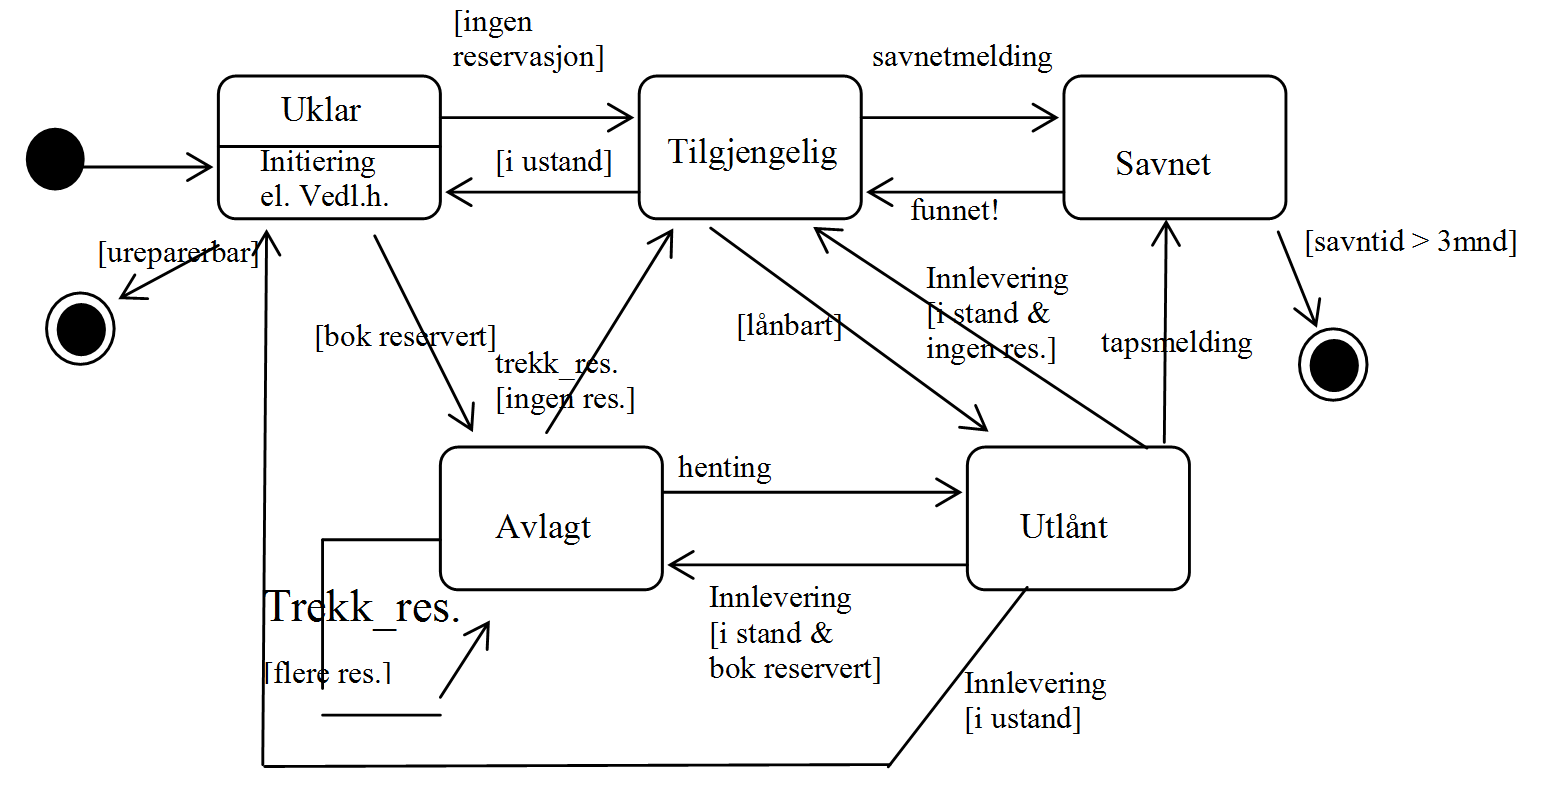
\includegraphics[scale=0.35]{resources/sequence-diagram-for-specimen-object.PNG}
    \caption{Tilstandsdiagram for eksemplar-objekt}
    \label{fig:sequence-diagram-for-specimen-object}
\end{figure}

\subsubsection{Tilstander}

Tilstander (eng. states) vises som firkanter med avrundede hjørner, og med navn som forklarer hva slags tilstand det er, dette vil typisk være adjektiver. Om man vil, kan man i stedet for selve tilstanden angi hvilken aktivitet som foregår mens objektet er i tilstanden, eller eventuelt angi både tilstand og aktivitet. Dette har vi gjort for tilstanden øverst til venstre, ”Uklar”. Et eksemplar vil befinne seg i denne tilstanden enten med det samme det er anskaffet, da man må initiere det (sette på strekkode og magnetstripe for tyverisikring), eller hvis slitasje gjør det nødvendig med vedlikehold. Således er aktiviteten her ”Initiering eller vedlikehold. Forøvrig har vi holdt oss til å kun navngi tilstander. ”Tilgjengelig”, ”Utlånt” og ”Savnet” burde være selvforklarende. ”Avlagt” innebærer at eksemplaret befinner seg i biblioteket, men er reservert av noen. Som vi husker fra klassediagrammet, gjaldt reservasjoner egentlig bøker, ikke eksemplarer, men den som har reservert, vil jo i så fall ønske det første eksemplaret biblioteket får kloa i, dette blir altså avlagt (f.eks. lagret ved disken, hvor låneren kan hente det).

\subsubsection{Start og stopp}
Start og stopp vises ved svarte rundinger, stopp med en hvit rand rund. Pilen fra Start-rundingen viser hvilken tilstand objektet vil befinne seg i når det oppstår, i dette tilfellet ”Uklart”. Piler som går til Stopp-rundinger viser fra hvilke tilstander objektet kan opphøre å eksistere, i dette tilfellet fra ”Uklar” og ”Savnet”.

\subsubsection{Overganger}
Overganger (eng. transitions) vises som piler mellom to tilstander, eller mellom en tilstand og start/stopp. Pilens retning forteller hvilken vei overgangen går, og den vil være annotert enten med navn på hendelsen som fører til overgangen og/eller en betingelse for når overgangen vil skje. Betingelser står i [ ]-parenteser, mens navn på hendelser står uten. I vårt eksempel er det altså noen overganger som bare har hendelsesnavn (f.eks. fra ”Tilgjengelig” til ”Savnet”) og noen som bare har betingelser (f.eks. fra ”Tilgjengelig” til ”Uklar”), og noen som har begge deler. Dette er valgfritt, man tar det som best illustrerer handlingsgangen.

Mens objektet tilbringer tid i de forskjellige tilstandene, er overgangene formelt sett ment å være momentane, dvs. ta null tid. Med hendelsen ”innlevering” mener man altså ikke hele handlingsgangen fra låneren kommer fram til disken og sier ”Jeg ønsker å levere inn denne boka” til innleveringen faktisk er blitt registrert og samtalen avsluttes med noen høflighetsfraser. Nei, her representerer hendelsen kun det øyeblikket akkurat da eksemplaret går fra å være utlånt til innlevert fra datasystemets synsvinkel, f.eks. ved at en statusverdi endres i databasen. Overgangen representerer altså kun det momentane skiftet av tilstand, ikke hva man gjør for å oppnå dette skiftet. Eventuelle betingelser innebærer derfor heller ikke at det gjøres noen vurderingen underveis på pilen (siden dette jo ville ta tid) – vurderinger av betingelser må eventuelt ha skjedd mens objektet fortsatt befant seg i fra-tilstanden.

Vårt eksempel kan nå forklares. Eksemplaret starter i den nevnte ”Uklar”-tilstanden. Når det er klargjort, vil det bli ”Tilgjengelig”, med mindre noen allerede har rukket å gjøre en reservasjon. I så fall blir eksemplaret ”Avlagt” (f.eks. lagret ved disken, i påvente av henting) for den som har reservert det. Når denne henter det avlagte eksemplaret, vil det bli ”Utlånt”, det samme skjer med et tilgjengelig eksemplar ved utlån. Her er betingelsen at eksemplaret er ”lånbart” – leksika og andre oppslagsverk vil det normalt være ulovlig å ta ut av biblioteket, men de er likevel tilgjengelige for studier på stedet. Når et utlånt eksemplar leveres tilbake, kan en av tre overganger inntreffe. Hvis eksemplaret er i ustand, sendes det på reparasjon, dvs. det blir ”Uklart” (dessuten må vi tro at låneren får et erstatningskrav, men dette vil ikke være med i vårt tilstandsdiagram, som bare tar for seg det som skjer med eksemplar-objektet). Hvis eksemplaret er i stand, og det ikke foreligger noen reservasjon av boken, vil det igjen bli tilgjengelig. Om det derimot fins en utilfredsstilt reservasjon for boken, vil det bli ”Avlagt”. Om den som har reservert, trekker reservasjonen tilbake, eller ikke henter eksemplaret innen en viss frist, blir det igjen ”Tilgjengelig”, med mindre det fins flere reservasjoner, da blir det ”Avlagt” til den neste i køen. Hvis en låner melder et eksemplar tapt, eller fortsatt ikke leverer etter et visst antall purringer, blir det ”Savnet”. Det samme kan skje med eksemplarer som ikke var utlånt, hvis man plutselig ikke finner dem på forventet plass biblioteket (kan være stjålet, feilplassert, feilaktig kastet, hvem vet?) Siden savnede eksemplarer kan dukke opp igjen, ønsker man ikke å slette objektet straks det meldes savnet eller tapt, i stedet venter man 3 måneder før man sletter objektet. Sletting kan også skje hvis man bestemmer seg for å kaste eksemplaret etter å ha funnet ut at det ikke lenger er verdt å reparere i tilstanden ”Uklar”.

Hvis tilstandsdiagrammene blir komplekse, kan det lønne seg å dekomponere dem, dvs. at noen tilstander kan ha sub-tilstander inni seg. I vårt første eksempel har vi overhodet ikke modellert komplikasjonene som inntreffer hvis en låner ikke returnerer et eksemplar i tide, annet enn at det til sist kan gå over til ”Savnet”. En mulighet kunne være å skille mellom to tilstander, en kalt ”Utlånt” som før, og en kalt ”Overlånt”, som innebærer at låneren har oversittet fristen. Hvis biblioteket har et fast system for purringer, f.eks. at man først venter til det har gått en uke over fristen, deretter sender ut første purring, så venter i ytterligere to uker før man sender ut andre purring, og deretter venter ytterligere tre uker før man sender siste purring, med beskjed om at låner må betale erstatning hvis man ikke leverer innen en uke. For en presis modellering kunne man her operere med en tilstand for hvert stadium i denne purringsprosessen. ”Overlånt” kan bety at fristen er utgått (men fremdeles med mindre enn en uke, slik at man ikke har purret ennå, hvilket innebærer at låneren kun får forsinkelsesgebyr, ikke purregebyr), deretter har man tilstandene ”Førstegangspurret”, ”Andregangspurret” og ”Sluttpurret”. Selvsagt kunne vi inkludere alle disse tilstandene på samme nivå som de vi allerede har i figur \ref{fig:sequence-diagram-for-specimen-object}, men dette ville bli nokså uoversiktlig. Et bedre alternativ er vist i figur \ref{fig:decomposed-state-example}, hvor vi som før har en ”Utlånt”-tilstand, bare at denne er dekomponert i fem sub-tilstander (”Normal”, som betyr at man fortsatt er innen fristen, pluss de fire stadiene av overskridelse).

\begin{figure}[H]
    \centering
    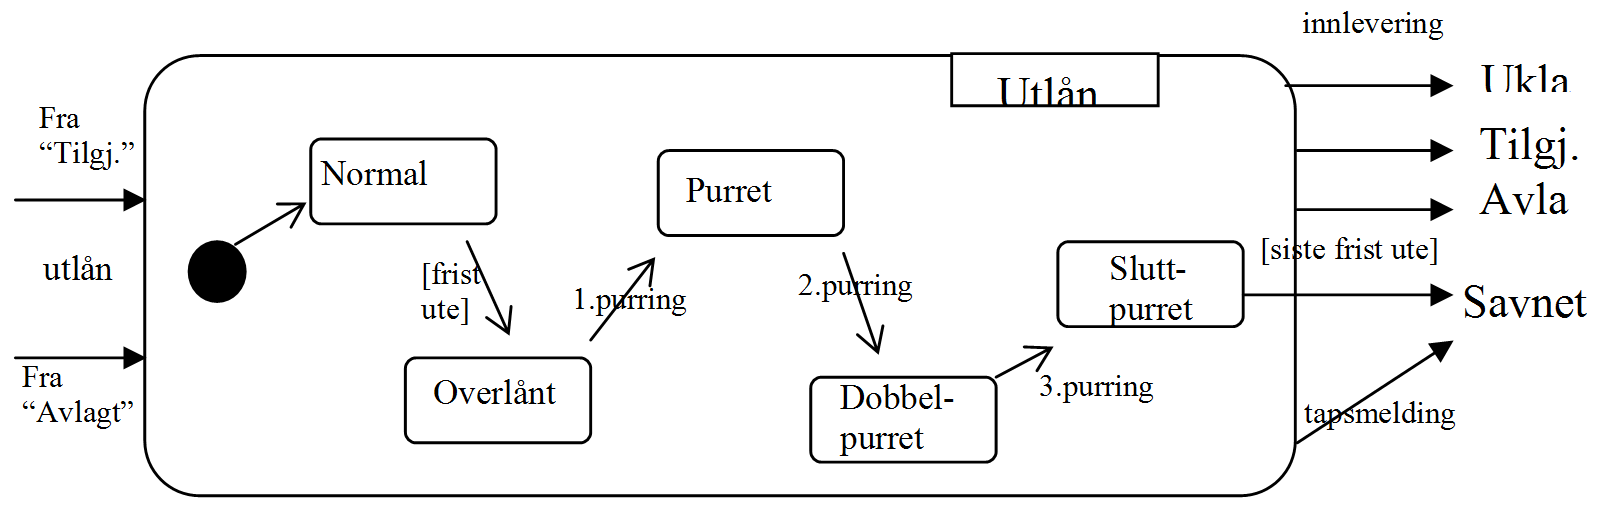
\includegraphics[scale=0.35]{resources/decomposed-state-example.PNG}
    \caption{En dekomponert tilstand}
    \label{fig:decomposed-state-example}
\end{figure}

Som vi ser går pilene på venstre side inn til supertilstanden ”Utlånt”, som er navngitt i et lite rektangel i kanten av den store boksen, og ikke til noen av subtilstandene. Da trenger vi et nytt start-symbol inni ”Utlånt”-tilstanden for å vise at man begynner i tilstanden ”Normal” (dvs. vanlig utlån, innen fristen). Alternativt kunne vi her ha kjørt pilene utenfra rett til ”Normal”, dette er en smakssak. Her har vi uansett ikke tjent noe i forhold til å modellere uten dekomponering. Fordelen med dekomponering kan derimot ses på høyre side. De tre pilene for ”innlevering” og den ene for ”tapsmelding” går her fra supertilstanden ”Utlånt” og ikke fra subtilstandene. Låneren kan jo på et hvilket som helst stadium i purreprosessen komme til å levere tilbake eksemplaret, eller melde det tapt. At pilene går fra supertilstanden indikerer nettopp dette, at overgangene kan skje uansett hvor man befinner seg inni den dekomponerte tilstanden. Hvis vi skulle ha modellert alle disse tilstandene uten bruk av dekomponering, måtte vi hatt tre innleveringspiler og en tapspil fra hver eneste av disse tilstandene. Dette ville gi et temmelig kaotisk diagram. Nå er det kun pilen til ”Savnet” i tilfelle låneren lar fristen gå ut uten å gi respons, som må gå fra en intern tilstand. Dette gjør ikke noe, for denne overgangen er kun aktuell fra ”Sluttpurret”, så den resulterer bare i en pil likevel.

Når man dekomponerer en tilstand i flere sub-tilstander, er det fortsatt meningen at objektet bare kan befinne seg i én av disse tilstandene om gangen. Men i noen tilfeller kan det også være interessant å operere med parallelle tilstander, hvor altså objektet kan være i flere tilstander på samme tid. Dette brukes når objektet kan gjennomgå flere forskjellige typer tilstandsendringer som er uavhengige av hverandre. Anta for eksempel at en bok kan være "Hyllet" (plassert i bibliotekets hyller, slik at lånere kan finne den selv) eller "Magasinert" (plassert i magasin, slik at det trengs en spesiell forespørsel til personellet for å få tak i den). En bok kan også være "Lånbar" eller "Ulånbar" (det siste vil gjerne være tilfelle for leksika og lignende, evt. også bøker som pga. alder eller sjeldenhet har nådd en betydelig verdi). For det tredje kan en bok være registrert som "Populær", "Middels" eller "Upopulær", alt etter hvor stor etterspørsel det er etter den (for eksempel basert på oppsamlede data, eller bibliotekspersonellets subjektive oppfatning). La oss her se bort ifra de eksakte kriteriene for at det skal skje endringer fra den ene tilstanden til den andre, men anta at de tre nevnte dimensjonene er uavhengige av hverandre. Dvs., en bok kan være "Hyllet, lånbar og populær", "Hyllet, lånbar og upopulær", "Magasinert, ulånbar og upopulær", etc., etc. Uten bruk av parallelle tilstander ville vi nettopp være nødt til å operere med slike komplekse tilstandsbetegnelser, og i alt ville vi få 12 tilstander (2 x 2 x 3).

For å unngå en kombinatorisk eksplosjon av tilstander når man har uavhengige alternativ, er det bedre å bruke parallelle tilstander. I UML er dette gjort ved å dele opp en tilstandsboks med stiplede linjer, hvert avdelt område tilsvarer da en parallell. Dette er vist i Figur \ref{fig:three-parallell-states-example}.

\begin{figure}[H]
    \centering
    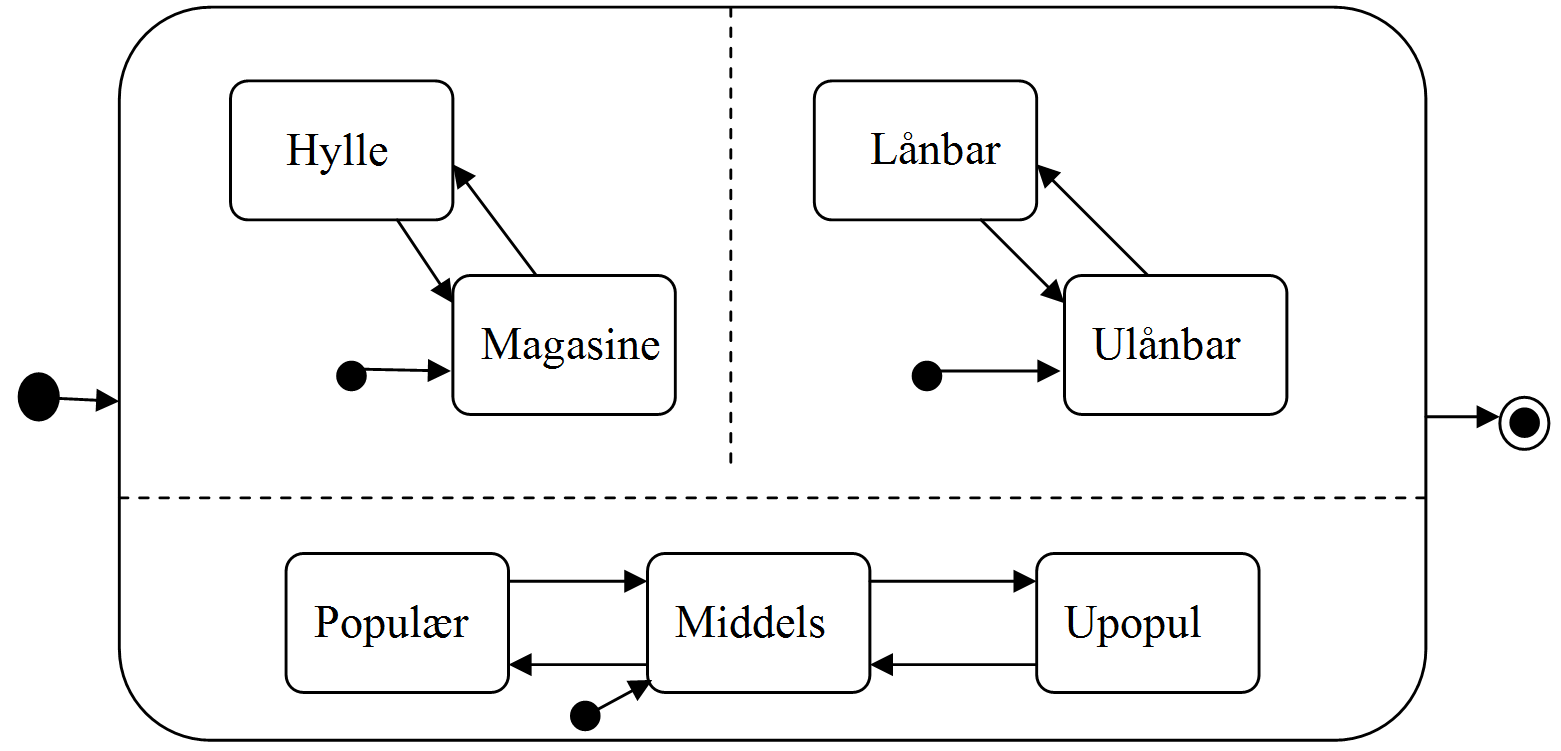
\includegraphics[scale=0.35]{resources/three-parallell-states-example.PNG}
    \caption{Tre parallelle tilstander}
    \label{fig:three-parallell-states-example}
\end{figure}

Aktivitetsdiagrammer kan oppfattes som en variant/utvidelse av tilstandsdiagrammer. Som nevnt i innledningen om tilstandsdiagrammer kunne vi inni en tilstandsboks navngi selve tilstanden og/eller den aktiviteten som foregikk i tilstanden. Aktivitetsdiagrammer vil altså være tilstandsdiagrammer der man kun, eller i hovedsak, opererer med aktiviteter. I den grad man fortsatt ønsker å inkludere selve tilstandsendringene i diagrammet, vil disse nå være vist som rektangler (med objektnavn, [tilstand]), koblet med stiplede piler til de aktiviteter som forårsaker tilstandsendringene. I tillegg har man en del andre konstruksjoner, f.eks. for å vise valgmuligheter, synkronisering og parallellprosessering.

For valg har man rombesymboler à la hva man vil være kjent med fra algoritmiske flytdiagrammer. I flytdiagrammer har man ofte bare to veier ut fra romben (f.eks. J og N, alt etter om betingelsen er sann eller usann), men i UMLs aktivitetsdiagrammer kan man ha piler ut, hver annotert med betingelsen for at denne skal velges, f.eks. [x<0], [x=0], [x>0]. Synkronisering og splitting vises begge ved en tykk stolpe som piler går inn til og ut fra. Flere piler inn og en ut betyr synkronisering – flere parallelle aktivitetstråder fortsetter i en felles. En pil inn og flere ut betyr splitting – en aktivitetstråd videreføres i flere parallelle aktiviteter. Denne symbolikken er vist i Figur \ref{fig:activity-diagram-notation-example}.

\begin{figure}[H]
    \centering
    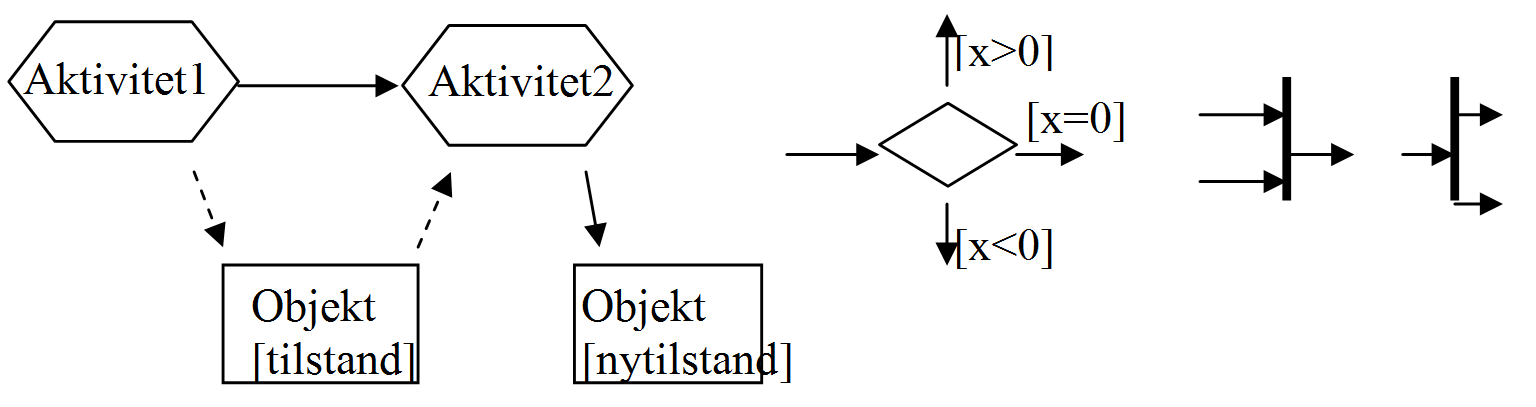
\includegraphics[scale=0.35]{resources/activity-diagram-notation-example.PNG}
    \caption{Notasjon for aktivitetsdiagrammer}
    \label{fig:activity-diagram-notation-example}
\end{figure}

Man trenger ikke ha med objekt/tilstandsbokser for hver aktivitet, bare hvis man finner dette nødvendig for diagrammets forståelighet. Hvis man bare bruker aktiviteter, vil diagrammet minne mye om tilstandsdiagrammer, piler indikerer overganger på samme måte, og man har samme symbolikk for start og stopp. For eksempler på bruk av aktivitetsdiagrammer, se nedennevnte støttelitteratur eller forelesning om tilstandsdiagrammer.

\subsection{Referanser}

Dette korte notatet har bare kunnet gi en rask innføring i UML, med det som er mest nødvendig for å komme i gang med prosjektet. For alle diagramtypene som er nevnt her, fins det mer avanserte muligheter som kunne ha vært nevnt i tillegg, ikke minst det formelle språket OCL, som kan brukes til tekstlige presiseringer i forhold til diagrammene, med formler, variabeltilordninger, betingelser o.l. Det fins dessuten en del diagramtyper som ikke er vist, f.eks. samarbeidsdiagrammer (collaboration diagrams), pakkediagrammer (package diagrams) og realiseringsdiagrammer (deployment diagrams). Pakkediagrammer, som viser hvordan store systemer er delt opp i moduler, vil man se et eksempel på i kravspesifikasjonen for prosjektet. For mer detaljer henviser vi til forelesninger og den nedennevnte støttelitteraturen.

\begin{enumerate}

\item
Martin Fowler, Kendall Scott: UML Distilled: applying the standard object-oriented modelling language, 1997, 179 s. (ordet distilled = destillert hentyder på en rask innføring, så kan man bare tenke seg hvor destillert dette lille notatet da må være).

\item
Rob Pooley, Perdita Stevens: Using UML: software engineering with objects and components, 1999, 254 s.

\item
Bernd Oesterreich: Developing Software with UML: object-oriented analysis and design in practice, 1999, 321 s.

\item
Charles Richter: Designing Flexible Object-Oriented Systems with UML, 1999, 404 s.

\item
Ivar Jacobson, Grady Booch, James Rumbaugh: The Unified Software Development Process, 1999, 463 s. (en bok av metodens/språkets opphavsmenn)

\item
Desmond F. D’Souza, Alan C. Wills: Objects, Components, and Frameworks with UML: the Catalysis Approach, 1999, 785 s.

\end{enumerate}
